\documentclass[11pt,a4paper,oneside,oldfontcommands]{ctexart}
\usepackage{tabularx}
\usepackage{array}
\usepackage{bm}
\usepackage{hyperref}
\usepackage{graphicx}
\usepackage{amsmath}
\usepackage{algorithm}
\usepackage{algpseudocode}
\usepackage{fancyhdr}
\pagestyle{fancy}

\hypersetup{hypertex=true,
	colorlinks=true,
	linkcolor=red,
	anchorcolor=blue,
	citecolor=blue}
\fancyhf{}
\chead{\textbf{算法设计与分析}}
\fancyhead[r]{\bfseries\thepage}
\fancyhead[l]{\bfseries\rightmark}
\renewcommand{\headrulewidth}{0.4pt} % 注意不用 \setlength
\renewcommand{\footrulewidth}{0pt}

\floatname{algorithm}{算法}
\renewcommand{\algorithmicrequire}{\textbf{输入:}}
\renewcommand{\algorithmicensure}{\textbf{输出:}}

\begin{titlepage}
	\title{\Huge\textbf{算法设计与分析 作业四}\\}
	\author{\Large\textbf{作者}:吴润泽 \and{\Large\textbf{学号}:181860109}\\
	\\
	\and {\Large\textbf{Email}:\href{mailto:181860109@smail.nju.edu.cn}{181860109@smail.nju.edu.cn}}\\}
	\date{\Large\today}
\end{titlepage}
\begin{document}
\maketitle
\newpage
\tableofcontents
\cleardoublepage
\section*{Chapter 4}
\markright{Chapter 4}
\addcontentsline{toc}{section}{Chapter 4}
{\subsection*{problem 4.2}}
\markright{problem 4.2}
\addcontentsline{toc}{subsection}{problem 4.2}
\hypertarget{(1)}{\subsubsection*{(1)}}
\textbf{$\Rightarrow$}如果w是v在DFS树中的后继结点,那么$actice(w)\subseteq active(v)$:\\
当$w\ne v$时,
因为w是v的后继结点,所以$v.discover<w.discover$,并且$v.finish>w.finish$。所以$actice(w)\subset active(v)$。当$w=v$时显然成立。
\textbf{$\Leftarrow$}如果$actice(w)\subseteq active(v)$,那么w是v在DFS树中的后继结点:\\
当$w\ne v$时,因为$active(w)\subseteq active(v)$,即$v.discover<w.discover$,并且$v.finish>w.finish$,即在遍历v的过程中将w遍历,即w是v的后继结点。
\hypertarget{(2)}{\subsubsection*{(2)}}
由\hyperref[(1)]{(1)}可知,w不是v的后继结点$\Leftrightarrow actice(w)\not\subset active(v)$。
v不是w的后继结点$\Leftrightarrow actice(v)\not\subset active(w)$得证。
\subsubsection*{(3)}
\paragraph*{\textcircled{1}}
\textbf{$\Rightarrow$}如果vw是CE,那么v和w没有祖先和后继关系,
由\hyperref[(2)]{(2)}可知active(w)和active(v)互不包含。同时CE说明在v指向w时,w已经是黑色结点,w已经遍历结束,
所以active(w)在active(v)之前。\\
\hspace*{20pt}\textbf{$\Leftarrow$ }active(w)在active(v)之前,w先完成整个遍历过程,后才遍历到v。且二者没有祖先后继关系,
那么边vw即为CE。\\
\paragraph*{\textcircled{2}}
\textbf{$\Rightarrow$}vw是DE,即v指向w时w为黑色,并且$active(w)\subset active(v)$,
若不存在第三个结点x,满足x是v的后继,w是x的后继,则v遍历到w时w一定为白色,边为TE。
即一定有$active(w)\subset active(x)\subset active(v)$。\\
\hspace*{20pt}\textbf{$\Leftarrow$}如果存在结点x,满足$active(w)\subset active(x)\subset active(v)$,
由\hyperref[(1)]{(1)}可知,x是v的后继,w是x的后继,且在遍历时v先走到x,然后x走到w,即v是w的祖先结点,因此vw是DE。\\
\paragraph*{\textcircled{3}}
\textbf{$\Rightarrow$}vw是TE,即v指向w时w为白色,w是v的后继,由\hyperref[(1)]{(1)}可知,$active(w)\subset active(v)$。
若存在x,满足$active(w)\subset active(x)\subset active(v)$,则在遍历时v先走到x,然后x走到w,
那么v是w的祖先而非父结点,与vw是TE矛盾。\\
\hspace*{20pt}\textbf{$\Leftarrow$}同理可得w是v的后继,且v直接指向w,则w是白色,即vw是TE。\\
\paragraph*{\textcircled{4}}
vw是BE$\Leftrightarrow$v是w的后继$\Leftrightarrow active(v)\subset active(w)$得证。\\

{\subsection*{problem 4.5}}
\markright{problem 4.5}
\addcontentsline{toc}{subsection}{problem 4.5}
\noindent \hypertarget{1.}{1. }不可能是TE。如果是TE,则有$active(v)\subset actice(u)$,即$v.finishTime>u.discoverTime$,故不成立。\\
2. 不可能是BE。如果是BE,则有$active(u)\subset actice(v)$,即$v.finishTime>u.discoverTime$,故不成立。\\
3. 不可能是DE。如果是DE,同样的v是u的后继结点,满足$active(v)\subset actice(u)$,同\hyperref[1.]{1.}不成立。\\
4. 可能是CE。
x结点先遍历v,然后从v返回x,x遍历u,易知$v.finishTime<u.discoverTime$。\\
如图所示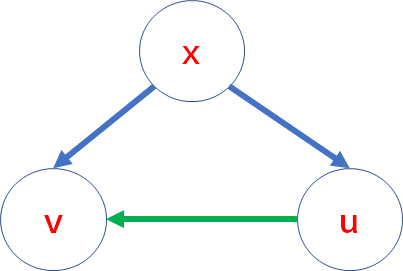
\includegraphics{CEORDER.png}\\
\newpage
{\subsection*{problem 4.7}}
\markright{problem 4.7}
\addcontentsline{toc}{subsection}{problem 4.7}
在第一次DFS中,将结点压栈,同一强连通片的源头结点是最后一个压栈的。\textbf{(引理4.4)}若l是某个强连通片首结点,x是另一个强连通片中的结点,
并且存在l通向x的路径,则x比l先结束遍历,即x先进栈l后进栈。满足这些性质,才能保证第二次DFS中,
按正确的顺序取出每个SCC的首结点。\\
\hspace*{20pt}无论是DFS还是BFS在一次遍历中都可以访问一个或者多个强连通片的所有结点。\\
\hspace*{20pt}如果第一次DFS换为BFS,由于BFS中按层序遍历,同一连通片中出度不为0的点可能先入栈。在第二次DFS的时候,不能有正确的访问顺序。
\hspace*{20pt}如果第二次DFS换为BFS,由于出栈的访问首结点顺序正确,BFS同样可以正确地划分强连通片。\\
\hspace*{20pt}因此第一次必须为DFS,第二次DFS和BFS都可以。
{\subsection*{problem 4.8}}
\markright{problem 4.8}
\addcontentsline{toc}{subsection}{problem 4.8}
\noindent\textbf{充要条件:}对于无向连通图的DFS生成树的根结点v,v是割点,当且仅当v有两个及两个以上的子树。
\paragraph{证明:}
\textbf{$\Rightarrow$}如果v是割点,假设v只有一个子树,易知子树是连通的,将v删除,
剩下的部分为v的子树仍然连通,这与v是割点相矛盾。因此v有两个及两个以上的子树。\\
\textbf{$\Leftarrow$}如果v有两个及两个以上的子树,因为图本身连通,则子树之间相连必然通过v,即v是割点。
{\subsection*{problem 4.9}}
\markright{problem 4.9}
\addcontentsline{toc}{subsection}{problem 4.9}
正确
\paragraph{证明:}
当从TE vw回退时,如果以w为根的子树存在BE指向v的祖先,
则v的祖先的discoverTime会被赋值给以w为根的子树中某个结点的back值,
并最终会传递到w.back,即必有$w.back<v.discoverTime$;\\
\hspace*{20pt}否则,没有存在BE指向v的祖先,如果子树不存在BE,则子树所有点back值均为初始值,
即$w.back>v.discoverTime$,如果子树中存在BE,则子树中的所有结点的back值也将大于等于$v.discoverTime$,
因为BE只能指向v或者子树内部结点,故back值最小也不会低于$v.discoverTime$,仍然满足$w.back>v.discoverTime$,即仍能正确判断是否为割点。
{\subsection*{problem 4.12}}
\markright{problem 4.12}
\addcontentsline{toc}{subsection}{problem 4.12}
算法中,默认环为多条TE和BE构成,但存在两条BE和TE构成环的情况。从A点出发,依次遍历B,C,D,E。
如下图所示。\\
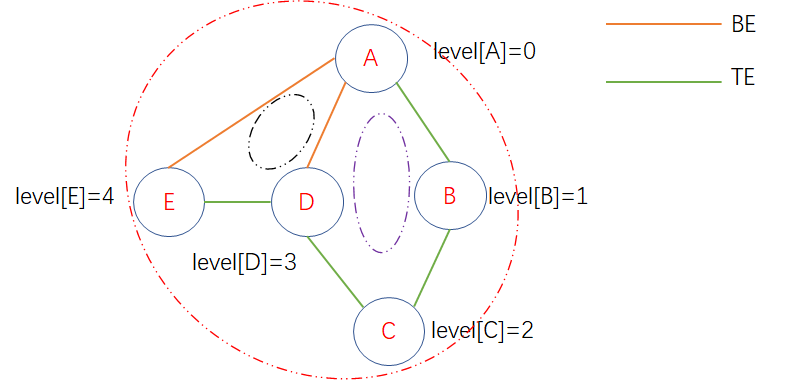
\includegraphics{4-12.png}\\
图中的BE为AE和AD,根据题目给定算法,计算出外圈大环的大小为5和右侧环大小为4,最终结果为4。
但图中最小环大小应为3,为左侧小环。因此算法不正确。
\newpage
{\subsection*{problem 4.13}}
\markright{problem 4.13}
\addcontentsline{toc}{subsection}{problem 4.13}
\paragraph{算法设计} 如果有向图没有环,则至少有一个点的入度为0。\\
1. 有向图中每个点的入度至少为1,则有图的边数不小于图的点数,则无向图中必定有环(存在BE)。\\
2. 利用DFS找到一条BE(找到一个环),设边为uv,u为后继,v为祖先。
(如果没有找到BE,说明存在一棵DFS生成树无环,则不能构造成功)\\
3. 以v为起点进行DFS,将每条TE xy,标记方向为x->y,最后将uv边标记方向为u->v,即满足了该环中每个点的入度都大于0。\\
4. 找到图中仍为白色的点,进行2、3步,若没有算法结束。\\
5. 由于只进行了两次深度优先遍历,较易得算法时间复杂度为线性。\\
\textbf{具体算法实现见}\hyperlink{AddDirection}{AddDirection算法}\\
$\begin{aligned}
		\hline
		\hypertarget{AddDirection}{}
		\label{AddDirection}
		 & \textbf{算法1 }AddDirection\text{ 算法}                                                             \\
		\hline
		 & 1.\textbf{Function}\ {FindLoop}\ (u)  \verb|\\|\text{找到一个环路,并返回BE边祖先结点} \\
		 & 2.\hspace*{20pt}u.color:=GRAY, res:=None                                                            \\
		 & 3.\hspace*{20pt}\textbf{foreach }neighbor\ v\ of\ u\textbf{ do}                                     \\
		 & 4.\hspace*{40pt}\textbf{if }v.color=WHITE\textbf{ and }v.vis=False\textbf{ then}                    \\
		 & 5.\hspace*{60pt}FindLoop(v)                                                                         \\
		 & 6.\hspace*{40pt}\textbf{elif }uv=BE\textbf{ then}                                                   \\
		 & 7.\hspace*{60pt}res:=u,\textbf{break}                                                               \\
		 & 8.\hspace*{20pt}\textbf{return }res                                                                 \\
		\hline
		 & 1.\textbf{Function}\ {AddDir}\ (u)    \verb|\\|\text{给环路加方向}                     \\
		 & 2.\hspace*{20pt}u.vis=True\verb|\\|\text{标记其已经加边避免重复}                       \\
		 & 3.\hspace*{20pt}\textbf{foreach }neighbor\ v\ of\ u\textbf{ do}                                     \\
		 & 4.\hspace*{40pt}\textbf{if }v.color=WHITE\textbf{ and }v.vis=False\textbf{ then}                    \\
		 & 5.\hspace*{60pt}change\ uv\ dircetion\ to\ u\rightarrow v                                           \\
		 & 6.\hspace*{60pt}AddDir(v)                                                                           \\
		 & 7.\hspace*{40pt}\textbf{elif }uv=BE\textbf{ then}                                                   \\
		 & 8.\hspace*{60pt}change\ uv\ dircetion\ to\ u\rightarrow v                                           \\
		\hline
		 & 1.\textbf{Function}\ {Main-AddDirection}\ (V,E)   \verb|\\|\text{wrapper部分}          \\
		 & 2.\hspace*{20pt}\textbf{foreach }point\ v\ in\ V\textbf{ do}                                        \\
		 & 3.\hspace*{40pt}v.color:=WHITE,v.vis:=False                                                         \\
		 & 4.\hspace*{20pt}\textbf{foreach }point\ v\ in\ V\textbf{ do}                                        \\
		 & 5.\hspace*{40pt}\textbf{if }v.color=WHITE\textbf{ and }v.vis=False\textbf{ then}                    \\
		 & 6.\hspace*{60pt}res:=FindLoop(v)                                                                    \\
		 & 7.\hspace*{60pt}\textbf{if }res=None\textbf{ then }\textbf{return }False                            \\
		 & 8.\hspace*{60pt}\textbf{else }AddDir(res)                                                           \\
		 & 9.\hspace*{20pt}\textbf{return }True                                                               \\
		\hline
	\end{aligned}
$\newpage
\hypertarget{problem 4.14}{\subsection*{problem 4.14}}
\markright{problem 4.14}
\addcontentsline{toc}{subsection}{problem 4.14}
\paragraph{证明 }有向无环图中必有入度为0的点。\\
\hspace*{20pt}设图有N个结点,假设每个点的入度均不为0,必有
$A_{2}\rightarrow A_{1},A_{3}\rightarrow A_{2},\cdots,A_{n}\rightarrow A_{n-1}$,
而对于$A_n$入度不为0,故存在某个结点指向它,则出现环路,产生矛盾,得证。\\
\textbf{算法设计}\\
0. 因为G是有向无环图,则G一定存在拓扑排序(\textbf{引理4.2})。\\
1. 入度最小的点(即拓扑排序的队首)a,如果图中存在哈密顿路径,则a的入度一定为0。假设a的入度不为0,结点x指向a。
由于a是拓扑排序队首,故一定存在a到达x的路径(因为有图连通)设为$a\rightarrow\cdots\rightarrow x$,同时x指向a,构成环路,与题干相矛盾。故a的入度一定为0。\\
2. 显然,从a点出发,如果存在哈密顿路径,则一次DFS遍历所有结点。\\
3. 首先找到图G的入度为0的点a,如果不存在或存在多个则不可能存在哈密顿通路。\\
4. 从a开始DFS,每当递归回溯时(边为uv),检查哈密顿路径path长度是否为结点个数。\\
5. 如果等于结点个数,说明存在路径$a\rightarrow\cdots u\rightarrow v\rightarrow\cdots n$,算法结束。\\
6. 否则,将$v.vis$置为假,将v从path中剔除(哈密顿通路上u不直接到达v),从u的下一子结点继续DFS。\\
7. 找最小入度结点为$O(m+n)$,DFS过程显然是$O(m+n)$,因此时间复杂度是线性的。\\
\textbf{具体算法实现见}\hyperlink{FindHamilton}{FindHamilton算法}\\
$\begin{aligned}
		\hline
		\hypertarget{FindHamilton}{}
		\label{FindHamilton}
		 & \textbf{算法2 }FindHamilton \text{ 算法}                                                                                             \\
		\hline
		 & 1.\textbf{Function}\ {FindHamilton}\ (u,path,n)  \verb|\\|\text{找到一个环路,并返回BE边祖先结点}                       \\
		 & 2.\hspace*{20pt}u.vis:=True,path.push(u)                                                                                             \\
		 & 3.\hspace*{20pt}\textbf{foreach }neighbor\ v\ of\ u\textbf{ do}                                                                      \\
		 & 4.\hspace*{40pt}\textbf{if }v.vis=False\textbf{ then}                                                                                \\
		 & 5.\hspace*{60pt}FindHamilton(v,path,n)                                                                                               \\
		 & 5.\hspace*{60pt}\textbf{if }len(path)==n\textbf{ then return }True                                                                   \\
		 & 6.\hspace*{60pt}v.vis:=False,path.pop()\verb|\\|\text{没有找到,故将vis置为假,将v从path剔除}                           \\
		 & 7.\hspace*{20pt}\textbf{return }False\verb|\\|\text{u所有子结点都没有找到哈密顿通路}                                    \\
		\hline
		 & 1.\textbf{Function}\ {Main-FindHamilton}\ (V,E)   \verb|\\|\text{wrapper部分}                                           \\
		 & 2.\hspace*{20pt}\textbf{foreach }point\ u\ in\ V\textbf{ do}                                                                         \\
		 & 3.\hspace*{40pt}u.vis:=False,u.cnt:=0\verb|\\|\text{入度初始化为0}                                                      \\
		 & 4.\hspace*{40pt}\textbf{foreach }neighbor\ v\ of\ u\textbf{ do }u.cnt++\verb|\\|\text{计算各点的入度}                  \\
		 & 5.\hspace*{20pt}tar:=None,cnt:=0  \verb|\\|\text{初始化要寻找的点}                                                     \\
		 & 6.\hspace*{20pt}\textbf{foreach }point\ u\ in\ V\textbf{ do}     \verb|\\|\text{找到唯一一个入度为0的点}               \\
		 & 7.\hspace*{40pt}\textbf{if }tar!=None\textbf{ and }cnt=0\textbf{ and }u.cnt=0                                                        \\
		 & 8.\hspace*{60pt}\textbf{ then return } False\verb|\\|\text{存在不止一个入度为0的点,不可能存在哈密顿通路}              \\
		 & 9.\hspace*{40pt}\textbf{if }cnt\geq u.cnt\textbf{ then }tar:=u,cnt:=u.cnt                                                            \\
		 & 10.\hspace*{15pt}\textbf{if }tar=None\textbf{ or }cnt!=0\textbf{ then return } False \verb|\\|\text{不存在入度为0的点} \\
		 & 11.\hspace*{15pt}\textbf{return }FindHamilton(tar)                                                                                   \\
		\hline
	\end{aligned}
$
\newpage
\markright{problem 4.16}
\hypertarget{problem 4.16}{\subsection*{problem 4.16}}
\addcontentsline{toc}{subsection}{problem 4.16}
\noindent 由\hyperlink{problem 4.14}{problem 4.14}证明可知,有向无环图必有入度为0的点。\\
\noindent\textbf{算法设计}\\
\textbf{1.} 有向无环图可以出现一个或者多个入度为0的结点,对这些结点的拓扑先后顺序没有要求。\\
\textbf{2.} 入度为0的结点的出边删去,必会出现入度为0的点(仍为无环图)。\\
\textbf{3.} 重复\textbf{1,2}步,直到算法结束。可知时间复杂度为线性。\\
由开始的\textbf{证明}可知,图中存在回路,会出现没有入度为0的点的情况,无法确定拓扑顺序。\\
\textbf{算法实现}\\
$\begin{aligned}
		\hline
		\hypertarget{ZeroTopoLogical}{}
		\label{ZeroTopoLogical}
		 & \textbf{算法3 }ZeroTopoLogical \text{ 算法}                                                                                                  \\
		\hline
		 & 1.\textbf{Function}\ {InitQueue}\ (G(V,E),queue)  \verb|\\|\text{找到一个环路,并返回BE边祖先结点}                             \\
		 & 2.\hspace*{20pt}\textbf{foreach }point\ u\ in\ V\textbf{ do}                                                                                 \\
		 & 3.\hspace*{40pt}\textbf{if }InEdge[u]=0\textbf{ then }                                                                                       \\
		 & 4.\hspace*{60pt}queue.push(u)                                                                                                                \\
		 & 5.\hspace{20pt}\textbf{return }len(queue)>0\verb|\\|\text{没有找到入度为0的点,返回False}                                      \\
		\hline
		 & 1.\textbf{Function}\ {Main-ZeroTopoLogical}\ (G(V,E))  \verb|\\|\text{找到一个环路,并返回BE边祖先结点}                        \\
		 & 2.\hspace*{20pt}queue.init(),topo:=list(),count:=0                                                                                           \\
		 & 3.\hspace*{20pt}\verb|/*|\text{queue存放入度为0的结点的队列,topo存放拓扑排序结果,count为排好序的结点数}\verb|*/| \\
		 & 4.\hspace*{20pt}\textbf{if }InitQueue(G,queue)=False\textbf{ then return} False                                                              \\
		 & 5.\hspace*{20pt}\textbf{while }queue.empty()!=False\textbf{ do}                                                                              \\
		 & 6.\hspace*{40pt}u=queue.pop(),topo[count++]=u\verb|\\|\text{确定u为当前的逻辑起点}                                             \\
		 & 7.\hspace*{40pt}\textbf{foreach }neighbor\ v\ of\ u\textbf{ do}                                                                              \\
		 & 8.\hspace*{60pt}InEdge[v]--                                                                                                                  \\
		 & 9.\hspace*{60pt}\textbf{if }InEdge[v]=0\textbf{ then }queue.push(v)                                                                          \\
		 & 11.\hspace{15pt}\textbf{return }count=len(V)\verb|\\|\text{所有结点应确定拓扑排序,否则存在环路}                               \\
		\hline
	\end{aligned}
$
\newpage
{\subsection*{problem 4.17}}
\markright{problem 4.17}
\addcontentsline{toc}{subsection}{problem 4.17}
\hypertarget{4.17(1)}{\subsubsection*{(1)}}
\noindent 易知只需要以顶点s为起点进行一次DFS,判断是否遍历所有点即可。代价为$O(m+n)$。\\
$\begin{aligned}
		\hline
		 & 1.\textbf{Function}\ {OneToAll}\ (G(V,E),s)                         \\
		 & 2.\hspace{20pt}DFS(s)                                               \\
		 & 3.\hspace*{20pt}\textbf{foreach }point\ u\ in\ V\textbf{ do}        \\
		 & 4.\hspace{40pt}\textbf{if }u.color=WHITE\textbf{ then return }False \\
		 & 5.\hspace*{20pt}\textbf{return }True                                \\
		\hline
	\end{aligned}$
\subsubsection*{(2)}
利用课本上的划分强连通片的算法,将有向图G改造为G的收缩图G$\downarrow$,
各点之间的方向转换为各连通片之间的方向,易知G$\downarrow$为有向无环图。\\
\hspace*{20pt}题目可以转换为一个连通片可以到达其他所有连通片。
由于G$\downarrow$为有向无环图,必有入度为0的连通片。
故如果图G存在到达所有顶点的点,其必在该连通片中。
再利用\hyperlink{4.17(1)}{(1)}算法判断该连通片能否到达所有连通片即可。\\
\hspace*{20pt}强连通片划分与DFS判断是否可达算法时间复杂度均为$O(m+n)$,因此时间复杂度为$O(m+n)$,符合题意。\\
\textbf{具体算法实现见}\hyperref[SccOneToAll]{SccOneToAll算法}\\
$\begin{aligned}
		\hline
		\label{SccOneToAll}
		 & \textbf{算法4 } \text{SccOneToAll 算法}                                                            \\
		\hline
		 & 1.\textbf{Function}\ {SccOneToAll}\ (G(V,E))                                                       \\
		 & 2.\hspace*{20pt}construct\ G\downarrow\ using\ Scc(G)                                              \\
		 & 3.\hspace*{20pt}point:=None,CountZero:=0\verb|\\|\text{记录入度为0的连通片个数}      \\
		 & 4.\hspace*{20pt}\textbf{foreach }point\ u\ in\ V\downarrow\textbf{ do}                             \\
		 & 5.\hspace*{40pt}\textbf{if }InEdge[u]=0\textbf{ then }                                             \\
		 & 6.\hspace*{60pt}point:=u,CountZero:=CountZero+1                                                    \\
		 & 7.\hspace*{20pt}\textbf{if }point=None\textbf{ or }CountZero>1\textbf{ then }                      \\
		 & 8.\hspace{40pt}\textbf{return }False\verb|\\|\text{没有或多个入度为0的点,返回False} \\
		 & 9.\hspace{20pt}\textbf{return }OneToAll(G\downarrow,point)                                         \\
		\hline
	\end{aligned}
$
\newpage
{\subsection*{problem 4.18}}
\markright{problem 4.18}
\addcontentsline{toc}{subsection}{problem 4.18}
\subsubsection*{(1)}
同样利用课本上的划分强连通片的算法,将有向图G改造为G的收缩图G$\downarrow$。
易知同一个连通片中的影响力值相同。
易得影响力最低的连通片,一定是出度为0的连通片(一定存在,可能只有一个连通片),影响力是连通片中结点个数减1。
因此,找到所有出度为0的连通片,并找出结点个数最小的即可。\\
\hspace*{20pt}SCC的划分和寻找出度为0的连通片并统计的时间复杂度为$O(m+n)。$\\
\textbf{算法实现}\\
$\begin{aligned}
		\hline
		\label{MinImpact}
		 & \textbf{算法5 } \text{MinImpact 算法}                                                                                  \\
		\hline
		 & 1.\textbf{Function}\ {MinImpact}\ (G(V,E))                                                                             \\
		 & 2.\hspace*{20pt}construct\ G\downarrow\ using\ Scc(G)                                                                  \\
		 & 3.\hspace*{20pt}MinPoint:=None,MinCount:=\infty\verb|\\|\text{记录连通片的最小个数}                      \\
		 & 4.\hspace*{20pt}\textbf{foreach }point\ u\ in\ V\downarrow\textbf{ do}                                                 \\
		 & 5.\hspace*{40pt}\textbf{if }OutEdge[u]=0\textbf{ and }MinImpact<number(u)\textbf{ then }                               \\
		 & 6.\hspace*{60pt}MinPoint:=u,MinCount:=number(u)                                                                        \\
		 & 7.\hspace{20pt}\textbf{return }(MinCount-1,MinPoint)\verb|\\|\text{结点个数减1为影响力,以及对应的连通片} \\
		\hline
	\end{aligned}
$
\subsubsection*{(2)}
同样得到有向图G的收缩图G$\downarrow$,易知影响力最大的连通片,一定是入度为0的连通片(压缩图无环)。\\
则对所有的入度为0的连通片进行DFS遍历,遍历到的连通片即为其可到达的,DFS结束后计算遍历到连通片的结点个数。
取所有DFS得到结点个数最多的即为所求。\\
由于每次DFS后,都要查找所有访问过的连通片,因此时间复杂度为$O(n(m+n))$。\\
\textbf{具体算法实现见}\hyperlink{MaxImpact}{MaxImpact算法}\\
$
	\begin{aligned}
		\hline
		\hypertarget{MaxImpact}{}
		\label{MaxImpact}
		 & \textbf{算法6 } \text{MaxImpact 算法}                                                                              \\
		\hline
		 & 1.\textbf{Function}\ {MaxImpact}\ (G(V,E))                                                                         \\
		 & 2.\hspace*{20pt}construct\ G\downarrow\ using\ Scc(G)                                                              \\
		 & 3.\hspace*{20pt}MaxPoint:=None,CurCount:=0,MaxCount:=0                                                             \\
		 & 4.\hspace*{20pt}\verb|/*|\text{记录最大的DFS生成树的根以及结点个数}\verb|*/|           \\
		 & 5.\hspace*{20pt}\textbf{foreach }point\ u\ in\ V\downarrow\textbf{ do}                                             \\
		 & 6.\hspace*{40pt}\textbf{if }InEdge[u]=0\textbf{ then }                                                             \\
		 & 7.\hspace*{60pt}DFS(G\downarrow,u),CurCount:=0   \verb|\\|\text{更新当前DFS树的结点个数}             \\
		 & 8.\hspace*{60pt}\textbf{foreach }point\ x\ in\ V\downarrow\textbf{ do}                                             \\
		 & 9.\hspace*{80pt}\textbf{if }x.vis=True\textbf{ then }                                                              \\
		 & 10.\hspace*{95pt}CurCount:=CurCount+number(x)                                                                      \\
		 & 11.\hspace*{95pt}x.vis:=False  \verb|\\|\text{将访问置为False,避免下次DFS错误计算}                  \\
		 & 12.\hspace*{55pt}\textbf{if }MaxCount<CurCount\textbf{ then }                                                      \\
		 & 13.\hspace*{75pt}MaxPoint:=u,MaxCount:=CurCount                                                                    \\
		 & 14.\hspace{15pt}\textbf{return }(MaxCount-1,MaxPoint)\verb|\\|\text{返回最大影响力,以及对应的连通片} \\
		\hline
	\end{aligned}
$
\newpage
\hypertarget{problem 4.20}{\subsection*{problem 4.20}}
\markright{problem 4.20}
\addcontentsline{toc}{subsection}{problem 4.20}
与\hyperlink{problem 4.16}{problem 4.16} 类似,每学期可以修所有入度为0的结点,将其加入暂存队列temqueue中。
0. 在安排课程数小于总课程数前,重复下列步骤。\\
1. 将temqueue的副本复制给queue,并将temqueue清空(避免每次都查找所有点来初始化队列)。\\
2. 将queue中的结点弹出,并将其指出的边删去,安排课程数加1。\\
3. 假设本题有解即为有向无环图,一定再次出现入度为0的结点,将其加入暂存队列temqueue中。\\
4. 当queue中结点全部弹出,学期数加1,即queue中的的课程均被安排。\\
可得算法时间复杂度是线性$O(m+n)$。\\
\textbf{算法实现}\\
$\begin{aligned}
		\hline
		 & \textbf{算法7 }ClassTopoLogical \text{ 算法}                                                                                                 \\
		\hline
		\label{ClassTopoLogClassical}
		 & 1.\textbf{Function}\ {Main-ClassTopoLogical}\ (G(V,E))  \verb|\\|\text{找到一个环路,并返回BE边祖先结点}                       \\
		 & 2.\hspace*{20pt}queue.init(),temqueue.init(),count:=0,TermCount:=0                                                                           \\
		 & 3.\hspace*{20pt}\verb|/*|\text{temqueue存放入度为0的结点的队列,count为排好序的结点数,TermCount为学期数}\verb|*/| \\
		 & 4.\hspace*{40pt}\textbf{if }\hyperref[ZeroTopoLogical]{InitQueue}(G,temqueue)=False\verb|\\|\text{初始化temqueue队列}          \\
		 & 5.\hspace*{60pt}\textbf{ then return }False  \verb|\\|\text{与\hyperref[ZeroTopoLogical]{problem 4.16 InitQueue函数}相同。}    \\
		 & 6.\hspace*{20pt}\textbf{while }count<len(V)\textbf{ do}\verb|\\|\text{安排的课程数还少于总课程}                                \\
		 & 7.\hspace*{40pt}queue:=temqueue.copy(),temqueue.clear()\verb|\\|\text{得到上一次记录的入度为0的结点}                           \\
		 & 8.\hspace*{40pt}\textbf{while }queue.empty()!=False\textbf{ do}                                                                              \\
		 & 9.\hspace*{60pt}u=queue.pop()                                                                                                                \\
		 & 10.\hspace*{55pt}count:=count+1\verb|\\|\text{已经确定的课程安排数加1}                                                         \\
		 & 11.\hspace*{55pt}\textbf{foreach }neighbor\ v\ of\ u\textbf{ do }                                                                            \\
		 & 12.\hspace*{75pt}InEdge[v]--                                                                                                                 \\
		 & 13.\hspace*{75pt}\textbf{if }InEdge[v]=0\textbf{ then }temqueue.push(v)                                                                      \\
		 & 14.\hspace*{35pt}TermCount:=TermCount+1\verb|\\|\text{安排的学期数加1}                                                         \\
		 & 15.\hspace{15pt}\textbf{return }TermCount\verb|\\|\text{最少的学期数}                                                          \\
		\hline
	\end{aligned}
$
\newpage
{\subsection*{problem 4.22}}
\markright{problem 4.22}
\addcontentsline{toc}{subsection}{problem 4.22}
\subsubsection*{(1)}
与\hyperlink{problem 4.16}{problem 4.16} 相同,i恨j记为i指向j。
找到合理的拓扑排序即可。如果存在环路则不存在拓扑排序。
仍为重复找入度为0的顶点u,将u放入拓扑序列中(因为没有人恨他),并删去u指向的边。
如果在所有点安排拓扑排序前,没有找到入度为0的顶点,说明存在环路,不存在符合条件的排队。\\
\textbf{具体算法实现}与\hyperref[ZeroTopoLogical]{ZeroTopoLogical算法}相同。
\subsubsection*{(2)}
与\hyperlink{problem 4.20}{problem 4.20} 相同。
首先将所有入度为0的点的边删除后,这些结点的行数记为row。
再将删除过程中发现的入度为0的点加入队列,row加1,表明开始下一次的排列。
重复上述过程,直到所有小孩被安排顺序。\\
\hspace*{20pt}如果没有发现入度为0的点且没有小孩全部安排,说明存在环路,不存在符合条件的安排。\\
\textbf{具体算法实现}与\hyperref[ClassTopoLogClassical]{ClassTopoLogClassical算法}相同。
{\subsection*{problem 4.23}}
\markright{problem 4.23}
\addcontentsline{toc}{subsection}{problem 4.23}
\noindent\textbf{(1)}
存在,$x_1=TRUE,x_2=TRUE,x_3=FALSE,x_4=TRUE$符合。\\
% \hypertarget{problem 4.23(2)}{\subsubsection*{(2)}}
\textbf{(2)}
$(x_3\vee x_4)\wedge(x_1\vee x_2)\wedge(\overline{x_1}\vee\overline{x_2})\wedge(\overline{x_1}\vee{x_2})\wedge({x_1}\vee\overline{x_2})$。
\subsubsection*{(3)}
\begin{figure}[h]
	\centering
	\begin{minipage}{150pt}
		\centering
		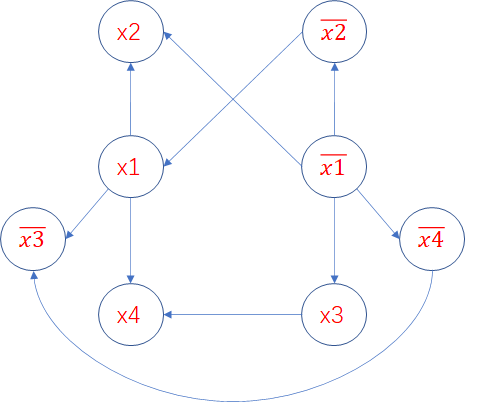
\includegraphics[width=150pt,height=120pt]{4-23-1.png}
		\caption{题目所给的实例}
	\end{minipage}
	\qquad
	\begin{minipage}{150pt}
		\centering
		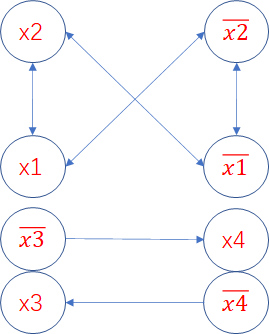
\includegraphics[width=100pt,height=120pt]{4-23-2.png}
		\caption{{(2)}中所给实例}
	\end{minipage}
\end{figure}
\subsubsection*{(4)}
\paragraph{证明}
如果连通片中存在同时包含$x$和$\overline{x}$的强连通片,
$(x\rightarrow \overline{x}),(x\leftarrow \overline{x})$两条边存在,
且由构造实例图过程
表明原2-SAT有子句$(x\wedge\overline{x})\equiv FALSE$,该子句恒为假,故实例I不存在使所有子句都满足的赋值。
\subsubsection*{(5)}
\paragraph{证明}
子句$(\alpha\vee\beta)\equiv (\overline{\alpha}\rightarrow \beta)
	\wedge(\overline{\beta }\rightarrow \alpha)$,因此若要使得$(\alpha\vee\beta)$成立,上述蕴涵关系必须成立。
在2-SAT实例图中的一条边$a\rightarrow b$则说明了必含有子句$(\overline{a}\vee b)$。故要想使得原式成立$a\rightarrow b$必须为TRUE。\\
\hspace*{20pt}因此可以抽象地看作,如果选取点a(a为TRUE),且存在$a\rightarrow b$,则b点必须选择。或者两者均不选择。
如果一系列结点在同一个强连通片中,意味着彼此可达,则要么都选择,要么都不能选择。
如果连通片中不存在一个文字及该文字的取反,说明这种选择是一定存在的。\\
\textbf{证明选择的可行性}\\
\hspace*{20pt}如果存在$a\rightarrow b$,则$\overline{b}\rightarrow\overline{a}$一定存在,即原图是存在对称关系的。
\hspace*{20pt}因此可以将原图化为强连通片压缩图G$\downarrow$(必为DAG),原图中的对称关系也存在于G$\downarrow$中。
即a所在连通片G1的其他文字的取反在$\overline{a}$的连通片$\overline{G1}$中。\\
\hspace*{20pt}对立连通片之间的对称传递:如果$G1\rightarrow G2$,那么$\overline{G2}\rightarrow \overline{G1}$。\\
\hspace*{20pt}同时对于DAG中存在边相连(祖先后继关系)的情况,为满足原式逻辑成立,故其后继也应为真,故需要进行拓扑排序。\\
\hspace*{20pt}因此,当x所在的强连通分量G1的拓扑序在$\overline{x}$所在的强连通分量的拓扑序之后则G1为真,$\overline{G1}$为假,
即按照反向拓扑的顺序进行(出度最小,对其它连通片影响最小)。重复选择直至所有连通片都被标记即可得到一组解。
\subsubsection*{(6)}
利用课本上的划分强连通片的算法,将有向图G改造为G的收缩图G$\downarrow$,之后进行逆向拓扑排序,即在构造图时将边的方向置反即可,
出度为0转化为入度为0。反复选取拓扑序在前的连通片并将其对立的连通片置为假即可。时间复杂度为线性$O(m+n)$。\\
\textbf{具体算法实现}\hyperref[2-SAT]{2-SAT算法}\\
$\begin{aligned}
		\hline
		\label{2-SAT}
		 & \textbf{算法8 } \text{2-SAT 算法}                                                                                                          \\
		\hline
		 & 1.\textbf{Function}\ {2-SAT}\ (G(V,E))                                                                                                     \\
		 & 2.\hspace*{20pt}queue.init(),temqueue.init(),count:=0                                                                                      \\
		 & 3.\hspace*{20pt}construct\ G\downarrow\ using\ Scc(G)                                                                                      \\
		 & 4.\hspace*{20pt}queue.init(),temqueue.init(),count:=0                                                                                      \\
		 & 5.\hspace*{20pt}\verb|/*|\text{temqueue存放入度为0的结点的队列,count为被选择的连通片个数}\verb|*/|             \\
		 & 6.\hspace*{20pt}\textbf{foreach }part\ X\ of\ V\downarrow\textbf{ do }                                                                     \\
		 & 7..\hspace*{40pt}\textbf{foreach }point\ y\ of\ X\downarrow\textbf{ do }                                                                   \\
		 & 8.\hspace*{60pt}\textbf{if }\overline{y} in X\textbf{ then return}FALSE                                                                    \\
		 & 9.\hspace*{40pt}\textbf{if }\hyperref[ZeroTopoLogical]{InitQueue}(G,temqueue)=False\verb|\\|\text{初始化temqueue队列}        \\
		 & 10.\hspace*{55pt}\textbf{ then return }False  \verb|\\|\text{与\hyperref[ZeroTopoLogical]{problem 4.16 InitQueue函数}相同。} \\
		 & 11.\hspace*{15pt}\textbf{while }count<len(V\downarrow)\textbf{ do}\verb|\\|\text{被选择的连通片个数}                         \\
		 & 12.\hspace*{35pt}queue:=temqueue.copy(),temqueue.clear()\verb|\\|\text{得到上一次记录的入度为0的结点}                        \\
		 & 13.\hspace*{35pt}\textbf{while }queue.empty()!=False\textbf{ do}                                                                           \\
		 & 14.\hspace*{55pt}u=queue.pop()                                                                                                             \\
		 & 15.\hspace*{55pt}\textbf{foreach }point\ x\ of\ u\textbf{ do }                                                                             \\
		 & 16.\hspace*{75pt}x.value=TRUE\verb|\\|\text{将u中所有点标记为TRUE}                                                           \\
		 & 17.\hspace*{55pt}count:=count+2\verb|\\|\text{已经确定连通片个数,对立连通片也被确认}                                        \\
		 & 18.\hspace*{55pt}\textbf{foreach }neighbor\ v\ of\ u\textbf{ do }                                                                          \\
		 & 19.\hspace*{75pt}InEdge[v]--                                                                                                               \\
		 & 20.\hspace*{75pt}\textbf{if }InEdge[v]=0\textbf{ then }temqueue.push(v)                                                                    \\
		 & 21.\hspace{15pt}\textbf{return }True\verb|\\|\text{能够正常选择}                                                             \\
		\hline
	\end{aligned}
$
\newpage
\section*{Chapter 5}
\markright{Chapter 5}
\addcontentsline{toc}{section}{Chapter 5}
{\subsection*{problem 5.1}}
\markright{problem 5.1}
\addcontentsline{toc}{subsection}{problem 5.1}
\subsubsection*{不存在BE}
假设存在边uv是BE,即当遍历结点u时,发现其黑色邻居v,且v是u在BFS树中的祖先结点。
由于为无向图,v也直接指向u,故当队列中v弹出时,发现u为白色,则将u加入队列,即vu是TE。
则在u出队时发现的uv边应是TE,不应二次遍历,故无向图BFS不存在BE。
\subsubsection*{不存在DE}
假设存在边uv是DE,在结点u刚出队列,即将处理它的所有邻居的时刻,结点v的情况:\\
1. 结点v不可能是白色,否则uv只能是TE。\\
2. 结点v不可能是灰色,因为u刚出队列,如果v为灰色,说明v已经在队列中,这和u是v在遍历树中的祖先结点矛盾。\\
3. 结点v不可能是黑色,在u刚被发现的时刻,如果v已经结束遍历,这同样与u是v在遍历树中的祖先结点矛盾。
{\subsection*{problem 5.2}}
\markright{problem 5.2}
\addcontentsline{toc}{subsection}{problem 5.2}
可以使用深度优先遍历判断。无向图DFS在遍历过程中如果uv为TE则直接给v染为与u相反颜色即可,
如果uv为BE说明存在环路,则判断uv两点颜色是否相同,若不同继续递归遍历,若相同则不是二分图。
$\begin{aligned}
		\hline
		\label{2-SAT}
		 & \textbf{算法9 } \text{BinaryDFS 算法}                                                                                                  \\
		\hline
		 & 1.\textbf{Function}\ {BinaryDFS}\ (u)
		 & 2.\hspace*{20pt}u.color:=GRAY, u.parcolor:=RED                                                                                         \\
		 & 3.\hspace*{20pt}\textbf{foreach }neighbor\ v\ of\ u\textbf{ do}                                                                        \\
		 & 4.\hspace*{40pt}\textbf{if }v.color=WHITE\textbf{ and }v.vis=False\textbf{ then}                                                       \\
		 & 5.\hspace*{60pt}v.parcolo:r=!u.parcolor\verb|\\|\text{给v添加与u相反的颜色}                                              \\
		 & 6.\hspace*{60pt}\textbf{if }BinaryDFS(v)=FALSE\textbf{ then return }FALSE                                                              \\
		 & 7.\hspace*{40pt}\textbf{elif }uv=BE\textbf{ then}                                                                                      \\
		 & 8.\hspace*{60pt}\textbf{if }u.parcolor=v.parcolor\textbf{ then return }FALSE\verb|\\|\text{如果uv颜色相同说明不是二分图} \\
		 & 9.\hspace*{20pt}\textbf{return }True \verb|\\|\text{可以正确染色}                                                        \\
		\hline
	\end{aligned}
$
\subsubsection*{深度优先遍历}
\noindent \textbf{优点:}能够找到所有的可行解,相比于BFS内存开销较小。\\
\textbf{缺点:}因为会发生回溯在深度较大的情况下效率不高。递归栈的空间与深度成正比存在爆栈的风险。
\subsubsection*{广度优先遍历}
\noindent\textbf{优点:}保证了每个结点只访问一遍,且以最短路径访问,效率高。\\
\textbf{缺点:}但是需要较大的内存来维护队列。
{\subsection*{problem 5.4}}
\markright{problem 5.4}
\addcontentsline{toc}{subsection}{problem 5.4}
\subsubsection*{(1)}
\noindent 对于一个结点,其高度为左右子树中较高子树的高度加1。
因此递归计算左右子树高度,当结点为空时高度记为0即可。每个结点访问一次,时间复杂度为$O(n)$。\\
$
	\begin{aligned}
		\hline
		 & 1.\textbf{Function}\ {MaxLen}\ (root)                        \\
		 & 2.\hspace*{20pt}\textbf{if }root=NULL\textbf{ then return }0 \\
		 & 3.\hspace*{20pt}left:=MaxLen(root->left)                     \\
		 & 4.\hspace*{20pt}right:=MaxLen(root->left)                    \\
		 & 5.\hspace*{20pt}\textbf{return }max(left,right)+1            \\
		\hline
	\end{aligned}
$
\subsubsection*{(2)}
\noindent 树的最短路径的最大的边一定通过根结点,
从根出发到达左子树最长边和到达右子树
最长边之和即为左右子树高度之和。时间复杂度同样为$O(n)$。\\
$
	\begin{aligned}
		\hline
		 & 1.\textbf{Function}\ {MaxWidth}\ (root)                      \\
		 & 2.\hspace*{20pt}\textbf{if }root=NULL\textbf{ then return }0 \\
		 & 3.\hspace*{20pt}left:=MaxLen(root->left)                     \\
		 & 4.\hspace*{20pt}right:=MaxLen(root->left)                    \\
		 & 5.\hspace*{20pt}\textbf{return }(left+right)                 \\
		\hline
	\end{aligned}
$
{\subsection*{problem 5.8}}
\markright{problem 5.8}
\addcontentsline{toc}{subsection}{problem 5.8}
\subsubsection*{(1)}
\subsubsection*{1. 有向图}
\paragraph{1.1 DFS }
\hypertarget{problem 5.8证明}{\textbf{证明:}}
有向图中,有环路当且仅当存在BE\\
在有向图中如果存在边uv是BE,说明v是u的祖先节点,
且有一条路径$v\rightarrow x\rightarrow \cdots\rightarrow u$,即u和v存在一条环路。
\\
如果有环,假设图中存在环路$u\rightarrow x\rightarrow\cdots v\rightarrow u$,
任取环路中一点y为起点进行DFS,且存在边wy,则在遍历中,当遍历至w时,发现有一条指向y的边,同时y是其祖先结点,故wy为BE。
\\
$
	\begin{aligned}
		\hline
		\label{DirDFSLoop}
		 & \textbf{算法10 } \text{DirDFSLoop 算法}     \\
		\hline
		 & 1.\textbf{Function}\ {DFSLoop}\ (u)  \verb|\\|\text{找到BE,返回True存在环路} \\
		 & 2.\hspace*{20pt}u.color:=GRAY                                                             \\
		 & 3.\hspace*{20pt}\textbf{foreach }neighbor\ v\ of\ u\textbf{ do}                                      \\
		 & 4.\hspace*{40pt}\textbf{if }v.color=WHITE\textbf{ then}                     \\
		 & 5.\hspace*{60pt}\textbf{if }DFSLoop(v)\textbf{ then return }True                                                                             \\
		 & 6.\hspace*{40pt}\textbf{elif }uv=BE\textbf{ then}                                                    \\
		 & 7.\hspace*{60pt}\textbf{return }True                                                               \\
		 & 8.\hspace*{20pt}\textbf{return }False                                                                  \\
		\hline
		 & 1.\textbf{Function}\ {DirDFSLoop}\ (V,E)   \verb|\\|\text{wrapper部分}          \\
		 & 2.\hspace*{20pt}\textbf{foreach }point\ v\ in\ V\textbf{ do}                                        \\
		 & 3.\hspace*{40pt}v.color:=WHITE     \verb|\\|\text{初始化所有点为未访问}                                                    \\
		 & 4.\hspace*{20pt}\textbf{foreach }point\ v\ in\ V\textbf{ do}                                        \\
		 & 5.\hspace*{40pt}\textbf{if }v.color=WHITE\textbf{ then}                    \\
		 & 6.\hspace*{60pt}\textbf{if }DFSLoop(v)\textbf{ then return }True \verb|\\|\text{存在环路,无需继续遍历}                                                                \\
		 & 7.\hspace*{15pt}\textbf{return }False    \verb|\\|\text{不存在返回False}                                                            \\
		\hline
	\end{aligned}
$
\newpage
\paragraph{1.2 BFS}
对于有向图,没有环,当且仅当存在拓扑排序。
由\hyperlink{problem 4.14}{problem 4.14}证明可知,有向无环图必有入度为0的点。
每次寻找入度为0的点将其加入队列,并按照BFS的方式进行遍历,
即队列每弹出一个结点,便将其出边删除,如果为无环图,该过程必产生入度为0的点,同样将其加入队列。
最后判断放入队列的结点数的个数,如果等于总结点数,说明无环,否则有环。\\
%\textbf{具体算法实现}与\hyperlink{ZeroTopoLogical}{ZeroTopoLogical算法}相同。\\
$
\begin{aligned}
	\hline
	\hypertarget{DirDFSLoop}{}
	\label{DirDFSLoop}
	 & \textbf{算法11 }DirBFSLoop \text{ 算法}                                                                                                  \\
	\hline
	 & 1.\textbf{Function}\ {BFSLoop}\ (u)  \verb|\\|\text{计算该次BFS可被安排的结点数}                        \\
	 & 2.\hspace*{20pt}queue.push(u),count:=0                                                                                           \\
	 & 3.\hspace*{20pt}\verb|/*|\text{queue存放入度为0的结点的队列,count为排好序的结点数}\verb|*/| \\
	 & 4.\hspace*{20pt}\textbf{while }queue.empty()!=False\textbf{ do}                                                                              \\
	 & 5.\hspace*{40pt}u=queue.pop(),count:=count+1\verb|\\|\text{确定u为当前的逻辑起点}                                             \\
	 & 6.\hspace*{40pt}\textbf{foreach }neighbor\ v\ of\ u\textbf{ do}                                                                              \\
	 & 7.\hspace*{60pt}InEdge[v]--                                                                                                                  \\
	 & 8.\hspace*{60pt}\textbf{if }InEdge[v]==0\textbf{ then }queue.push(v)                                                                          \\
	 & 9.\hspace*{20pt}\textbf{return }count\verb|\\|\text{返回排好序的结点数}                               \\
	\hline
	 & 1.\textbf{Function}\ {DirBFSLoop}\ (G(V,E))  \verb|\\|\text{wrapper部分}                             \\
	 & 2.\hspace*{20pt}count:=0 \verb|\\|\text{count为排好序的结点数}\\
	 & 3.\hspace*{20pt}\textbf{foreach }point\ u\ in\ V\textbf{ do}                                                                                 \\
	 & 4.\hspace*{40pt}\textbf{if }InEdge[u]=0\textbf{ then }                                                                                       \\
	 & 5.\hspace*{60pt}count:=count+BFSLoop(u)                                                                                                                \\
	 & 6.\hspace*{20pt}\textbf{return }count=len(V)>0\verb|\\|\text{所有结点应确定拓扑排序,否则存在环路}                                      \\
	\hline
	\end{aligned}
$
\newpage
\subsubsection*{2. 无向图}
\paragraph{2.1 DFS}
对于无向图,DFS中可能出现BE和TE,由\hyperlink{problem 5.8证明}{1.1DFS}证明可知,如果有BE则有环路。\\
$
	\begin{aligned}
		\hline
		\label{NoDirDFSLoop}
		 & \textbf{算法12 } \text{NoDirDFSLoop 算法}     \\
		\hline
		 & 1.\textbf{Function}\ {NoDFSLoop}\ (u)  \verb|\\|\text{找到BE,返回True存在环路} \\
		 & 2.\hspace*{20pt}u.color:=GRAY                                                             \\
		 & 3.\hspace*{20pt}\textbf{foreach }neighbor\ v\ of\ u\textbf{ do}                                      \\
		 & 4.\hspace*{40pt}\textbf{if }v.color=WHITE\textbf{ then}                     \\
		 & 5.\hspace*{60pt}\textbf{if }NoDFSLoop(v)\textbf{ then return }True                                                                             \\
		 & 6.\hspace*{40pt}\textbf{else return }True\verb|\\|\text{不是TE,则有环路}                                                                                                                \\
		 & 7.\hspace*{20pt}\textbf{return }False                                                                  \\
		\hline
		 & 1.\textbf{Function}\ {NoDirDFSLoop}\ (V,E)   \verb|\\|\text{wrapper部分}          \\
		 & 2.\hspace*{20pt}\textbf{foreach }point\ v\ in\ V\textbf{ do}                                        \\
		 & 3.\hspace*{40pt}v.color:=WHITE      \verb|\\|\text{初始化所有点为未访问}                                                   \\
		 & 4.\hspace*{20pt}\textbf{foreach }point\ v\ in\ V\textbf{ do}                                        \\
		 & 5.\hspace*{40pt}\textbf{if }v.color=WHITE\textbf{ then}                    \\
		 & 6.\hspace*{60pt}\textbf{if }NoDFSLoop(v)\textbf{ then return }True \verb|\\|\text{存在环路,无需继续遍历}                                                                \\
		 & 7.\hspace*{15pt}\textbf{return }False    \verb|\\|\text{不存在返回False}                                                            \\
		\hline
	\end{aligned}
$
\newpage
\paragraph{2.2 BFS}
对于无向图,BFS中可能存在CE和TE,如果存在uv为CE,即当遍历u时刻发现v是灰色,即两者皆在队列中,那么u和v必有一点x(已经出队)可达,
则三点构成环路。\\
$
\begin{aligned}
	\hline
	\hypertarget{DirDFSLoop}{}
	\label{DirDFSLoop}
	 & \textbf{算法13 }NoDirBFSLoop \text{ 算法}                                                                                                  \\
	\hline
	 & 1.\textbf{Function}\ {NoBFSLoop}\ (u)  \verb|\\|\text{找到一个环路,并返回BE边祖先结点}                        \\
	 & 2.\hspace*{20pt}queue.push(u),u.color:=GRAY                                                                                        \\
	 & 3.\hspace*{20pt}\verb|/*|\text{queue存放入度为0的结点的队列}\verb|*/| \\
	 & 4.\hspace*{20pt}\textbf{while }queue.empty()!=False\textbf{ do}                                                                              \\
	 & 5.\hspace*{40pt}u=queue.pop()\verb|\\|\text{确定u为当前的逻辑起点}                                             \\
	 & 6.\hspace*{40pt}\textbf{foreach }neighbor\ v\ of\ u\textbf{ do}                                                                              \\
	 & 7.\hspace*{60pt}\textbf{if }v.color=WHITE\textbf{ then }queue.push(v)                                                                          \\
	 & 8.\hspace*{60pt}\textbf{else return }True\verb|\\|\text{存在其他边,则为环路}\\
	 & 9.\hspace*{20pt}\textbf{return }False\verb|\\|\text{当前BFS生成树不存在环路}                               \\
	\hline
	 & 1.\textbf{Function}\ {NoDirBFSLoop}\ (G(V,E))  \verb|\\|\text{wrapper部分}                             \\
	 & 2.\hspace*{20pt}\textbf{foreach }point\ v\ in\ V\textbf{ do}                                        \\
	 & 3.\hspace*{40pt}v.color:=WHITE   \verb|\\|\text{初始化所有点为未访问}                                                     \\
	 & 4.\hspace*{20pt}\textbf{foreach }point\ u\ in\ V\textbf{ do}                                                                                 \\
	 & 5.\hspace*{40pt}\textbf{if }u.color=WHITE\textbf{ then }                                                                                       \\
	 & 6.\hspace*{60pt}\textbf{if }NoBFSLoop(u)\textbf{ then return }True  \verb|\\|\text{存在环路,无需继续遍历}                                                                                                               \\
	 & 7.\hspace*{20pt}\textbf{return }False\verb|\\|\text{不存在返回False}                                      \\
	\hline
	\end{aligned}
$
综上无论是DFS还是BFS,不存在环路当且仅当仅有TE边。
\subsubsection*{(2)}

{\subsection*{problem 5.9}}
\markright{problem 5.9}
\addcontentsline{toc}{subsection}{problem 5.9}
{\subsection*{problem 5.10}}
\markright{problem 5.10}
\addcontentsline{toc}{subsection}{problem 5.10}
\end{document}